\documentclass{article}

\usepackage[utf8]{inputenc}
\usepackage[T1]{fontenc}      
\usepackage[francais]{babel}
\usepackage{graphicx}
\usepackage{circuitikz}
\usepackage[squaren, Gray]{SIunits}
\usepackage{sistyle}
\usepackage[autolanguage]{numprint}
\usepackage{pgfplots}
\usepackage{amsmath,amssymb,array}
\usepackage{url} 

% New command pour la modélisation mécanique, tri à effectuer
\newcommand\fv[1]{{\bf #1}} % free vector
\newcommand\fvd[1]{\dot{\bf #1}} % free vector derivated
\newcommand\fvdd[1]{\ddot{\bf #1}} % free vector derivated
\newcommand\fvr[1]{\mathring{\bf #1}} % free vector relatively derivated
\newcommand\fvrr[1]{\overset{\circ\circ}{\bf #1}} % free vector relatively derivated
\newcommand\uv[1]{{\bf\hat{ #1}}} % unit vector
\newcommand\ui{{\bf\hat{I}}} % unit vector I
\newcommand\uj{{\bf\hat{J}}} % unit vector J
\newcommand\uk{{\bf\hat{K}}} % unit vector K
\newcommand\wrt[2]{\ensuremath{\tensor*[_{ #1}]{ #2}{}}} % With Respect To
\newcommand\wtr[3]{\ensuremath{\tensor*[_{ #1}]{ #2}{^{ #3}}}} % With Two Respect
\newcommand\omegaf{{\bm \omega}}
\newcommand\omegafr{\mathring{\bm \omega}}
\newcommand\omegafd{\dot{\bm \omega}}
\newcommand\omegaft{\tilde{\bm \omega}}
\newcommand\omegaftr{\mathring{\tilde{\bm \omega}}}
\newcommand\omegat{\tilde{\omega}}
\newcommand\omegatd{\tilde{\dot{\omega}}}
\newcommand\ine{{\bf I}}
\newcommand\st{{\bf L}}
\newcommand\pst{{\bf M}}
\newcommand\lm{{\bf N}}
\newcommand\am{{\bf H}}
\newcommand\amd{\dot{\am}}
\newcommand\fo{{\bf F}}
\newcommand\po{\mathcal{P}}
\newcommand\xg{\ensuremath{\fv{R}}}
\newcommand\xgd{\ensuremath{\fvd{R}}}
\newcommand\xgdd{\ensuremath{\fvdd{R}}}
\newcommand\dvec[1]{\dot{\vec{ #1}}}
\newcommand\ddvec[1]{\ddot{\vec{ #1}}}
\newcommand\qp{\dot{q}}
\newcommand\dqp{\Delta \dot{q}}

\begin{document}


% La description de l’appareillage de mesure est claire et complète
\section{Description de l'appareillage}
Afin de tester le circuit de notre haut-parleur, nous avions besoin d'une alimentation
capable de fournir du $\unit{\pm 15}{\volt}$ (pour alimenter le dual ampli-op ainsi
que l'amplificateur audio). Nous avions donc besoin de deux alimentations DC Topward 
\numprint{3303} DS présente au laboratoire. Pour obtenir une tension négative par 
rapport à une tension de référence, il faut connecter ensemble les deux chassis,
et les bornes $+$ de la première source, et $-$ de la deuxième source. La première règle
alors la tension négative et la deuxième la tension positive\cite{dctopward}.
Au niveau de l'intensité du courant, étant donné que la puissance maximale de l'amplificateur
audio est de \unit{2.5}{\watt}\cite{datasheetampli} et que la tension d'alimentation est de \unit{15}{\volt}, par
la formule $P = VI$ en utilisant la valeur RMS, on obient \unit{0.23}{\ampere}. Nous règlons
donc les deux sources sur cette valeur. Les cables des deux alimentation sont ensuite connectés 
aux bornier de la plaquette. La sortie de la plaquette est quant à elle relier à la bobine mobile.

L'électroaimant est lui alimenté en courant continu par une troisième source qui 
fourni un courant de \unit{1}{\ampere}. Le courant maximum supporté par les fils de 
cuivre dont nous disposons étant de \unit{2}{\ampere}\cite{norme-cuivre}, nous prenons
une bonne marge de sécurité afin d'éviter la surchauffe des fils.

Enfin, pour les différentes mesures, nous utilisons :

\begin{itemize}
	\item Un oscilloscope lorsque nous désirons le signal passant par un point de notre circuit ;
	\item Un multimètre pour mesurer un courant, une tension ou une résistane ;
	\item Un teslamètre pour mesurer l'intensité du champ magnétique produit par notre électroaimant.
\end{itemize}

\section{Compte-rendu des mesures}

\subsection{Mesures du champ magnétique produit par l'électroaimant}
Pour mesurer le champ magnétique produit par l'électroaimant, nous nous servons du teslamètre.
Le champ qui nous intèresse se situe dans l'entrefer de l'électroaimant, il suffit alors de placer
la sonde du teslamètre dans cet entrefer. Il est difficile d'obtenir une mesure très précise en se
servant du teslamètre car la valeur qu'il nous indique n'est pas très stable. Cependant, en répétant
plusieurs fois l'expérience et en notant les valeurs affichées par le teslamètre, on obtient une mesure
moyenne de \unit{8}{\centi\tesla} ; un résultat qui confirme nos prédictions théoriques
qui annonçait un champ magnétique de \unit{7.54}{\centi\tesla}.

\subsection{Mesures en différents points du circuit}
Pour mesurer la tension du signal audio en différent point du circuit, nous utilisons l'oscilloscope
et sa sonde.

\paragraph{Point d'entrée}

\paragraph{}

%La méthode des mesures est expliquée

%Nous avons fait des mesures de voltage en fonction de différentes fréquences pour les filtres RC: ce qui nous a permis
%de trouver les fréquences de coupures. Pour mesurer les différentes valeurs reprises ci dessous, nous avons procédé de la
%façon suivante: nous avons branché deux générateurs à la plaquette: Une source positive branchée à la borne $+15$ de la plaquette.
%Une source négative branchée à la borne $-15$ de la plaquette. La terre est quant à elle branchée au dernier point
%disponible de la plaquette: gnd (pour ground). De plus, la terre est branchée aux sources positives et négatives
%restantes. Quand nous mesurons la tension aux différents points nous nous servons d'un oscilloscope. Avec la sonde,
%nous touchons le circuit où nous voulons savoir la valeur de la tension. Sur l'écran, on voit apparaitre le
%signal, en réglant l'appareil sur le bon ordre de grandeur, nous pouvons mesurer assez précisement la tension en
%tel ou tel point. En annexe, on peut voir des photos des phases de tests.
  %Nous avons fait ces tests avec les filtres
%passe haut et passe bas. Cela correspond au bloc 1 et 2.
%
%\begin{figure}[ht!]
    %\centering
    %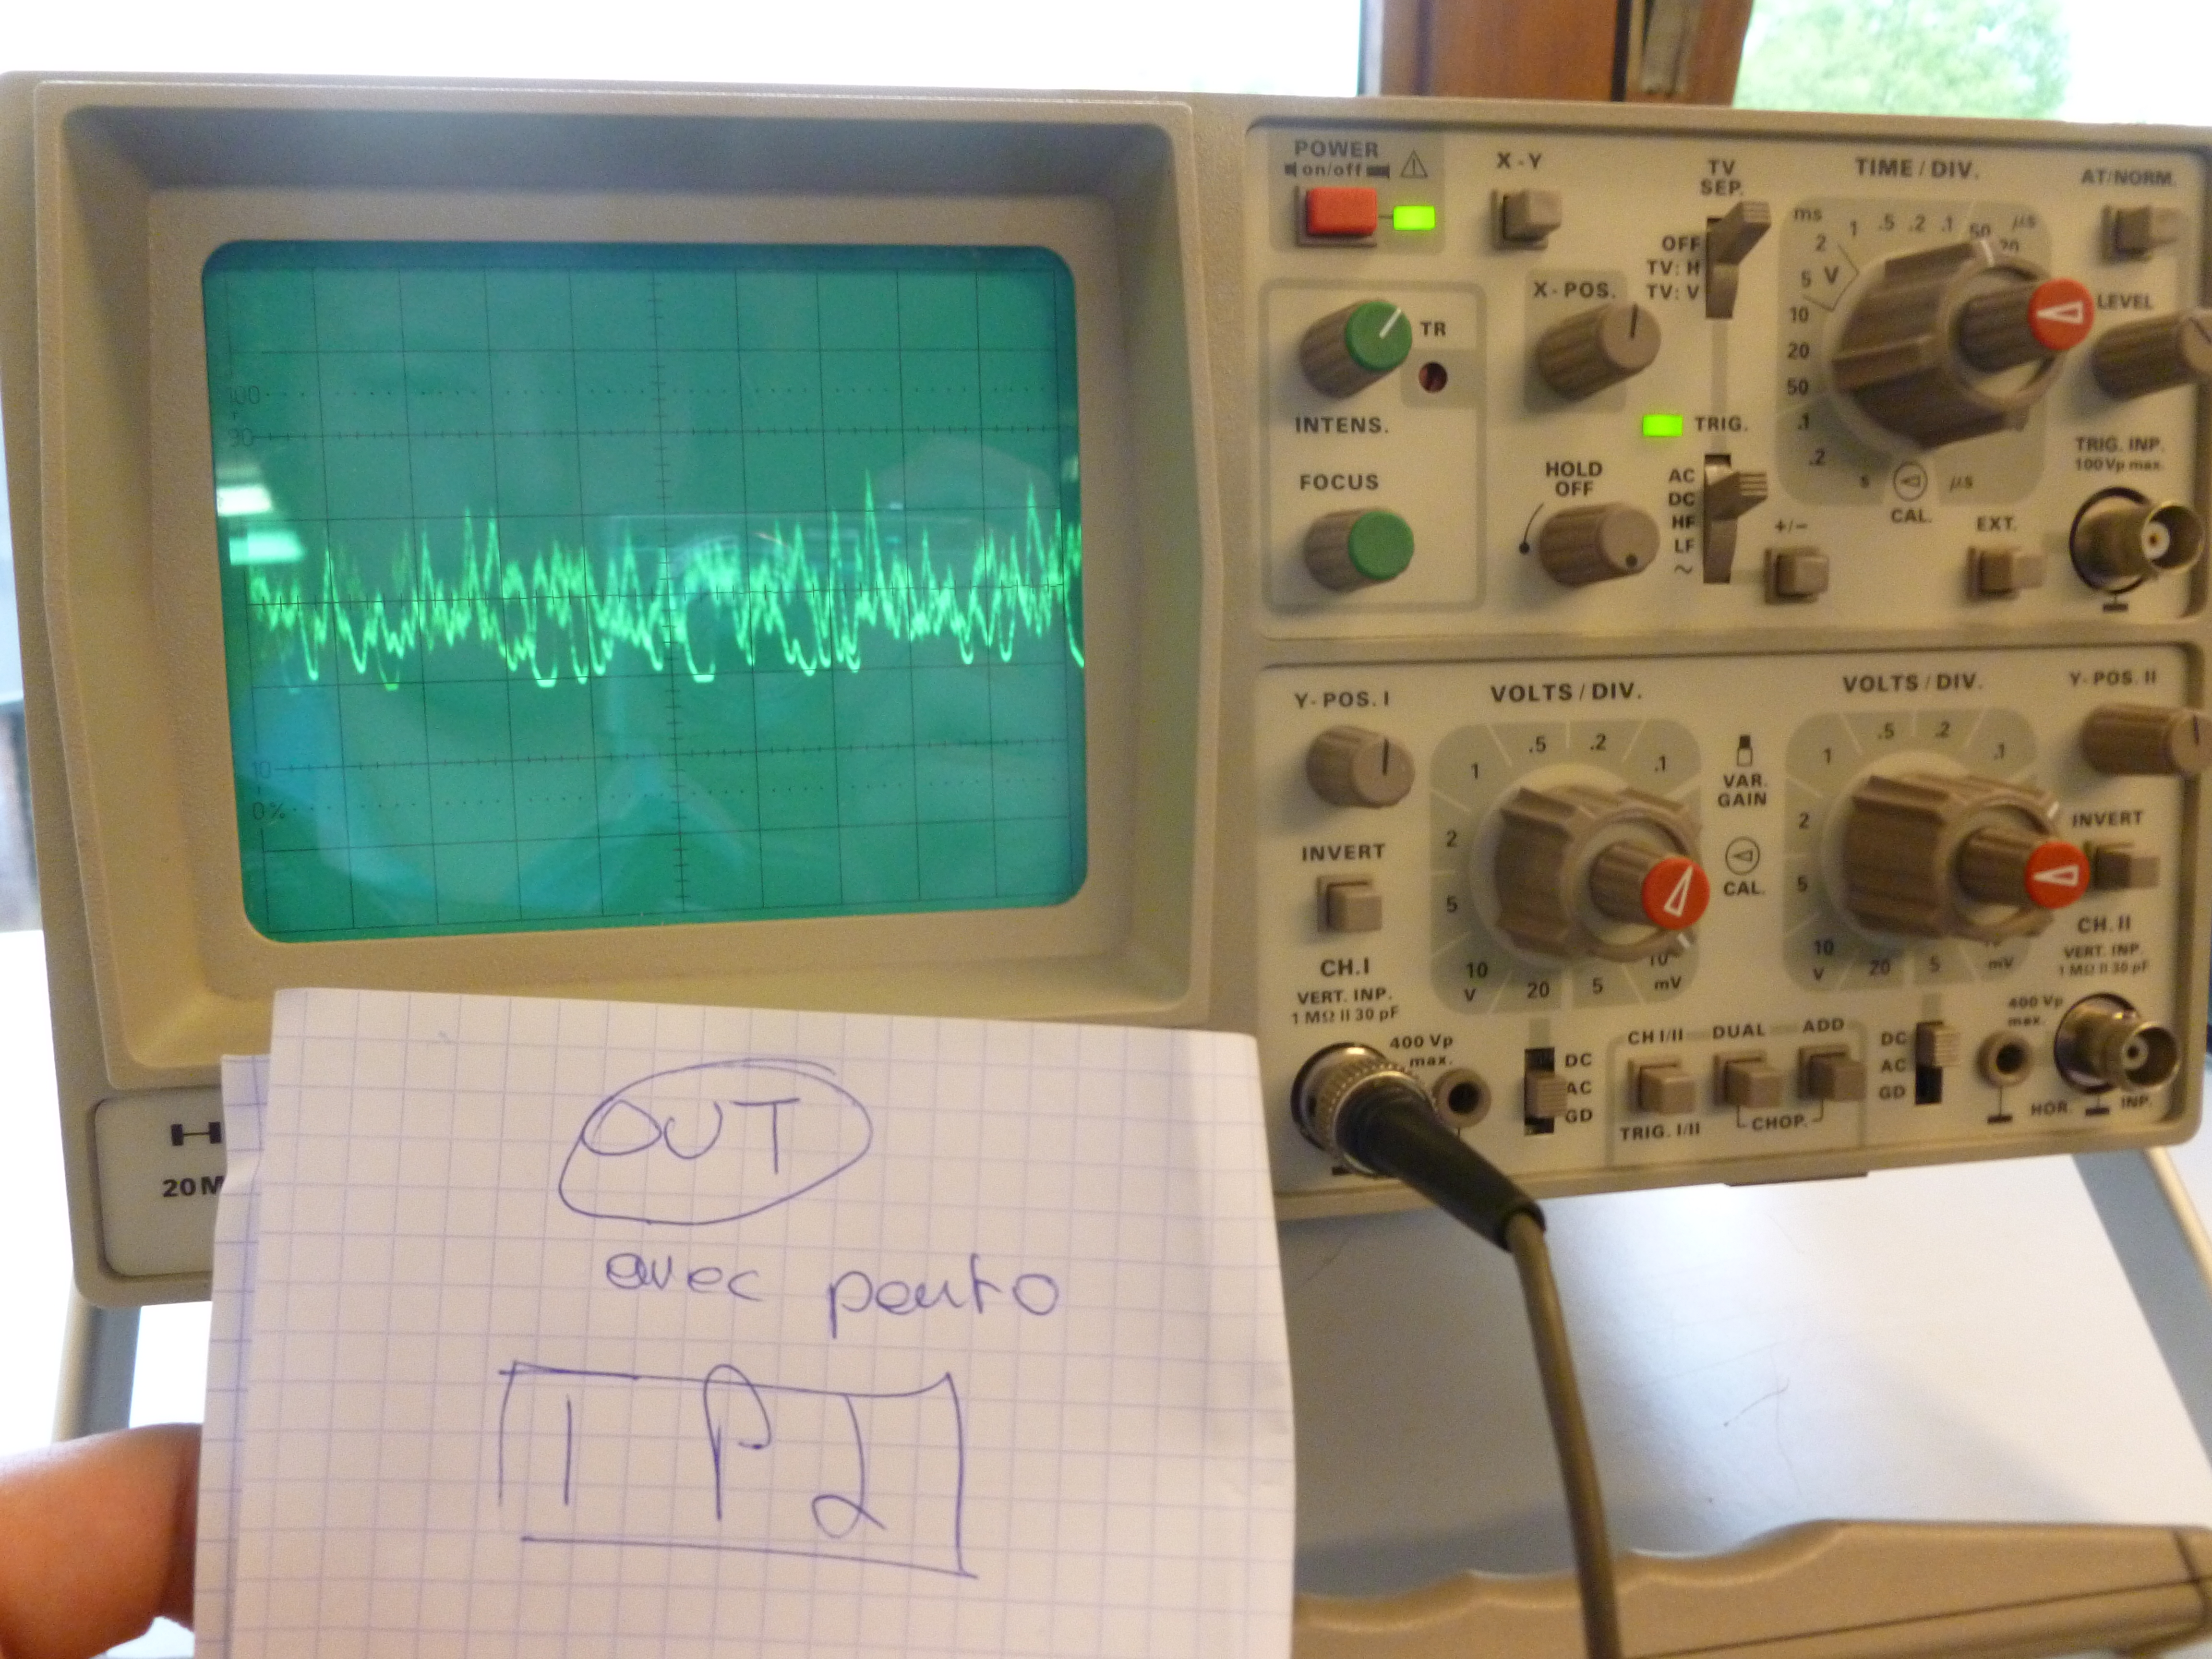
\includegraphics[scale=0.05]{P1010038.jpg}
    %\caption{Oscilloscope}
    %\label{Oscilloscope pour TP2}
%\end{figure}
%
%%Des tests paramétriques sont effectués
%Nous avons décidé de faire nos essais avec une tension de plus et moins 15 V car l'ampli-op nécéssite une tension
%de maximum plus et moins 16.5 V, nous prenons un peu moins pour avoir une marge de sécurité.
%Il est clair que si nous changeons cette valeure et que nous mettons plus de tension, le son sera plus amplifié vu que
%la plaquette aura une plus grande source de tension.
%
%
%En faisant augmenter les aigus, nous voyons que le signal est plus condensé et vice versa.
%
%Quand nous mettons plus de courant dans la bobine fixe, un plus grand champs magnétique est créé, mais trop l'augmenter
%ferait fondre le fil.
%
%\begin{figure}[ht!]
    %\centering
    %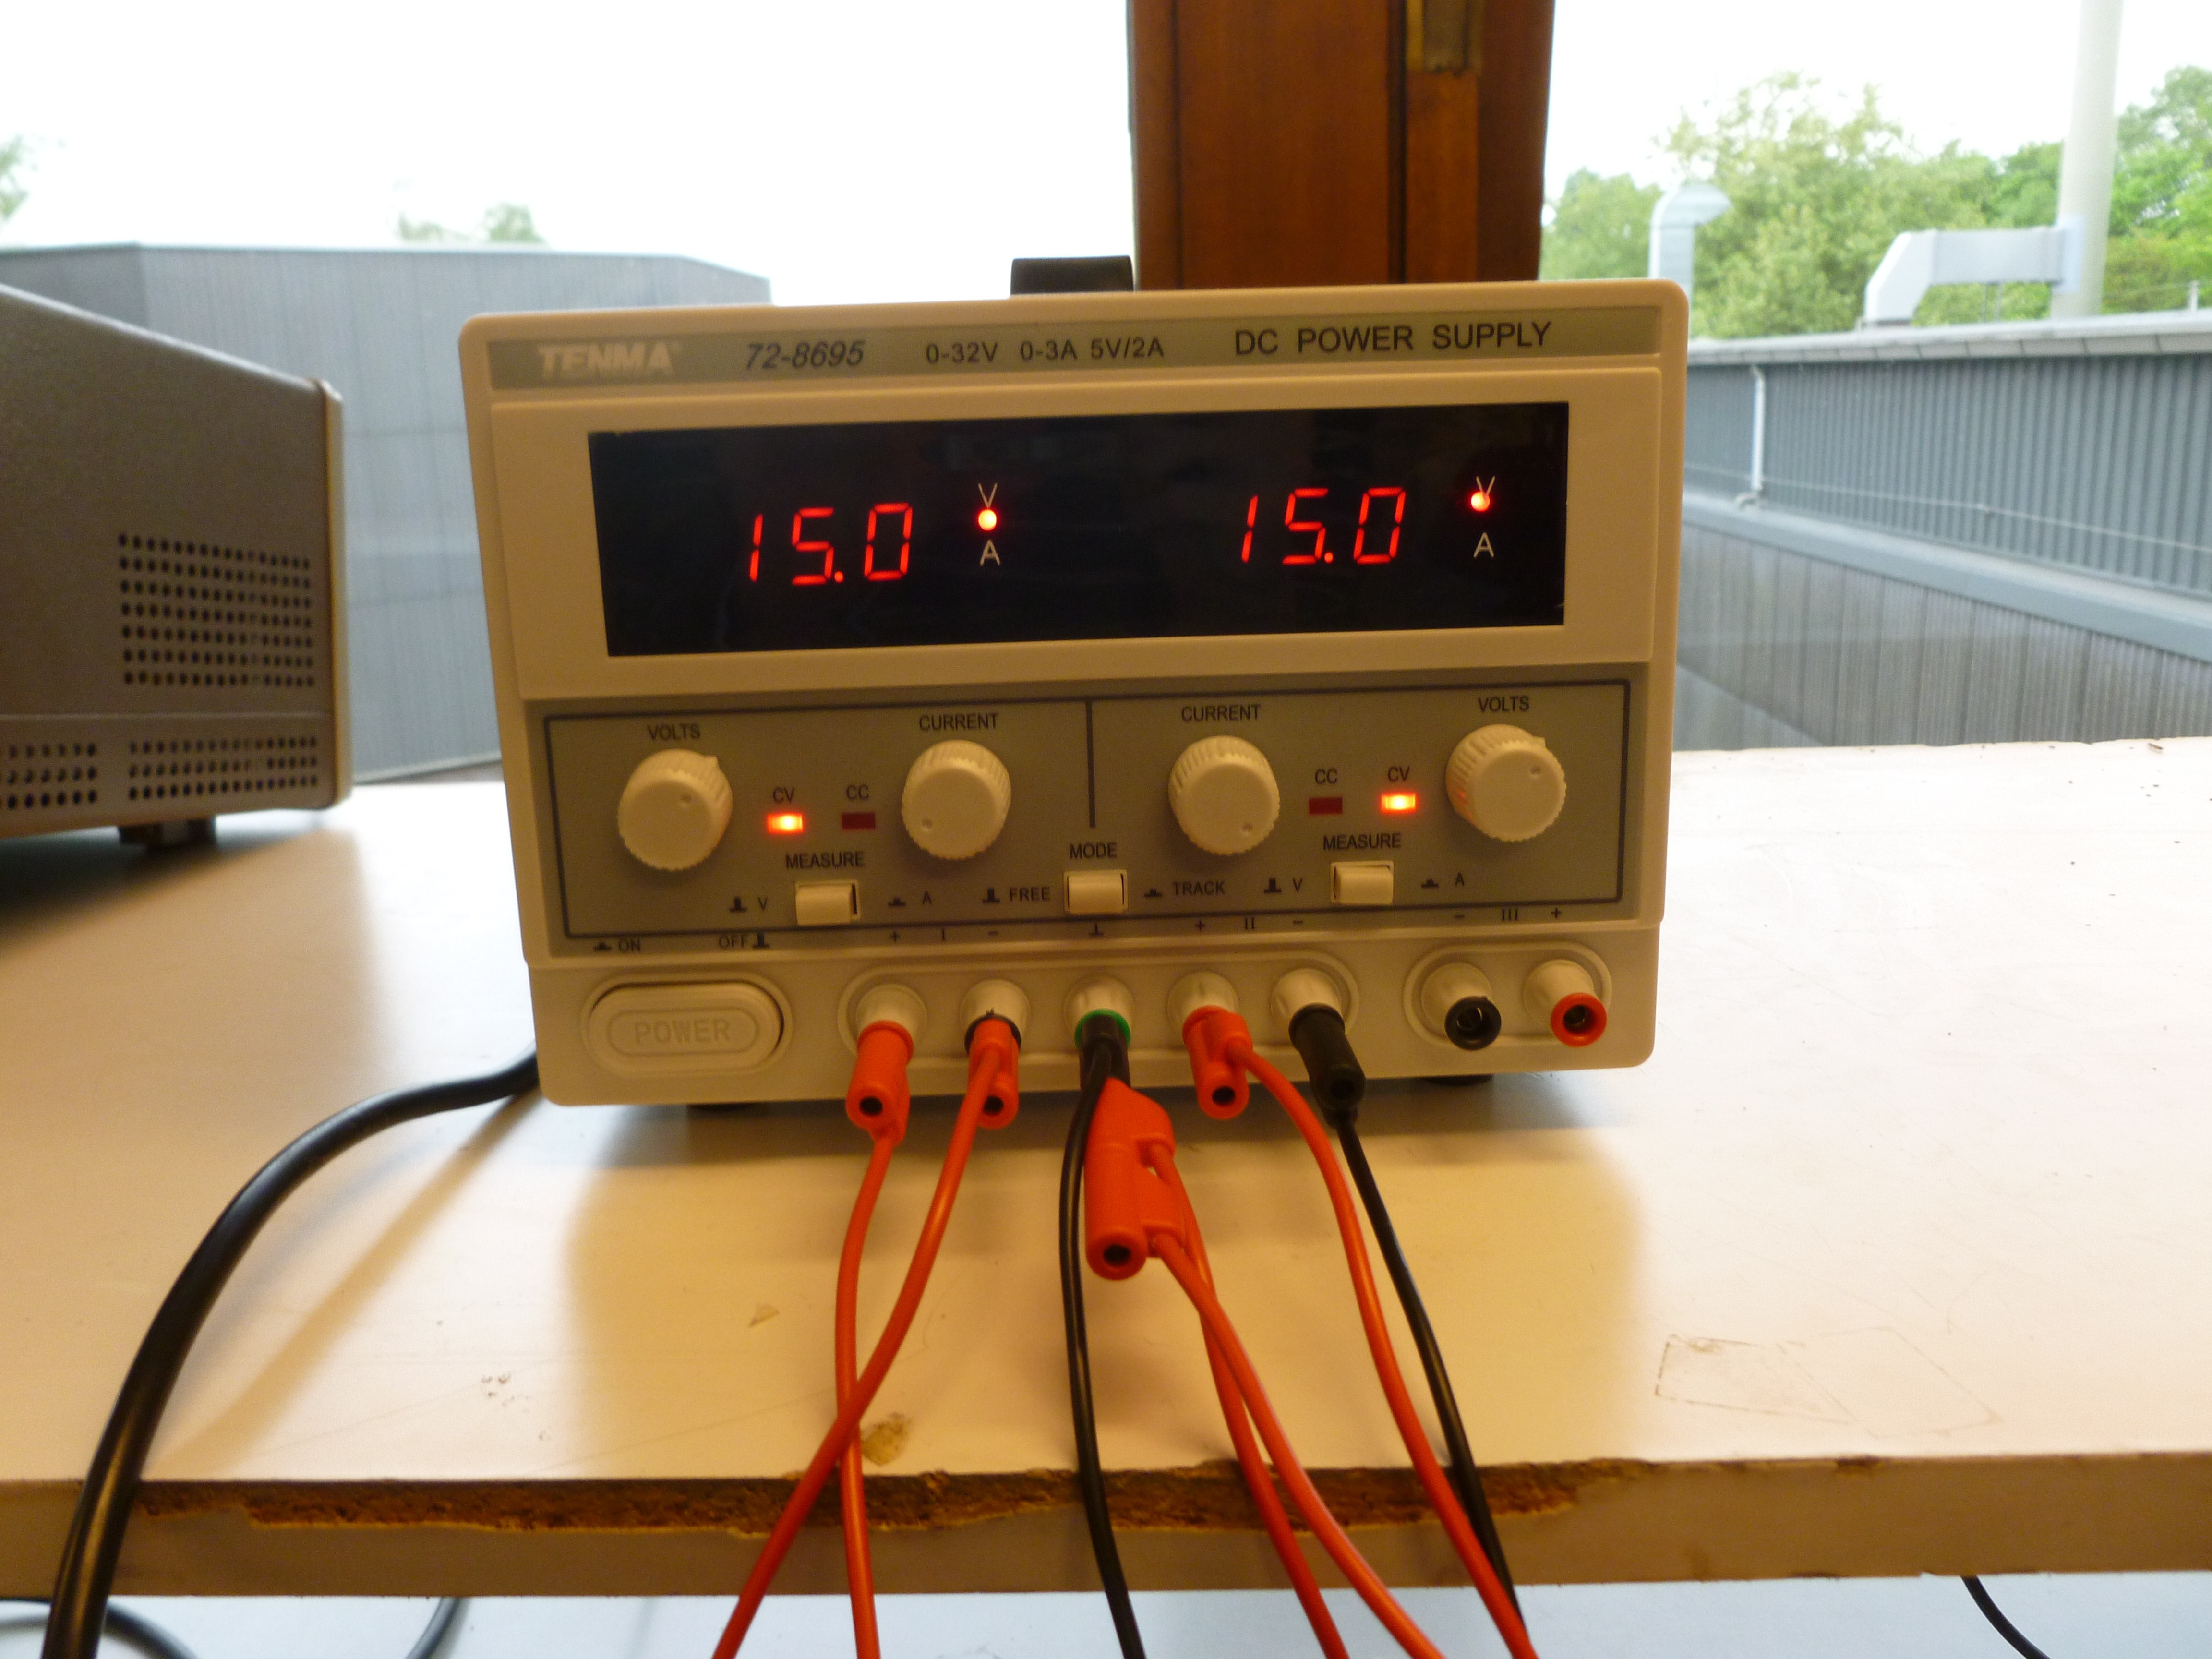
\includegraphics[scale=0.05]{P1010031.jpg}
    %\caption{Générateurs}
    %\label{Branchements des générateurs}
%\end{figure}
%
%%Mesures
%Pour le filtre passe-bas:
%\begin{center}
%\begin{tabular}{|c|c|c|}
%\hline
%$V_c[V]$ & $f[Hz]$ & $\log{f}$ \\
%\hline
%1.7 & 16000 & 4.204 \\
%\hline
%1.55 & 18000 & 4.255 \\
%\hline
%1.45 & 20000 & 4.301 \\
%\hline
%\end{tabular}
%\end{center}
%
%
%
%\begin{center}
%\begin{tabular}{|c|c|c|}
%\hline
%"Resistance bobine fixe[\ohms]" & "Champ magn.[T]" & "Amperage[A]" \\
%\hline
%2.38 & 0.08 & 0.1667\\
%\hline
%\end{tabular}
%\end{center}
%
%\begin{document}
%
%\begin{center}
%\begin{tabular}{|c|c|c|c|c|}
%\hline
%"Prise Jack [mV]" & "IN_1 [mV]" & "OUT_{avec pentotiomètre} [V]" & "OUT_{sans pentotiomètre} [V]" & $TP_2 [mV]$ \\
%\hline
%37.5 & 100.0 & 0.22 & 3.0 & 11.0 \\
%\hline
%\end{tabular}
%\end{center}

% Just here to fix rapport_prejury.tex
\end{document}
